\documentclass[12pt]{article}
\usepackage[lmargin=1in,rmargin=1in,tmargin=1in,bmargin=1in]{geometry}

\usepackage{aryaman}

\setcounter{tocdepth}{2}

\title{Linear Quotients of Connected Ideals of Graphs}
\author{Aryaman Maithani (Joint work with H. Ananthnarayan and Omkar Javadekar)}
\date{February 16, 2024}

\usepackage[
	hyperref = true,      	% Link to online documents
  	backend  = bibtex,      % Use bibtex instead of biber
  	sorting  = nyt,       	% Sorts by (name, year, title)
  	style  = alphabetic 	% Citations look like [Har77]
]{biblatex}
\addbibresource{talks.bib}

\begin{document}

\maketitle
% \tableofcontents

\section{Introduction}

Notes I made for my talk at BIKES -- the student commutative algebra seminar at the University of Utah. I introduce the notions of linear resolutions and linear quotients, as well as some monomial ideals related to graphs. I mention our results of characterising when the connected ideals of trees have linear quotients, and giving a sufficient condition for general graphs.

\section{Monomial ideals}

Throughout the talk, $K$ will denote an arbitrary field, and $R$ will be a polynomial ring over $K$.

\begin{defn}
	A \deff{monomial ideal} is an ideal of $R$ generated by monomials.
\end{defn}

\begin{ex}
	$I \vcentcolon= (ab, bc, ca) \subset K[x, y, z]$ is a monomial ideal.
\end{ex}

A rich source of monomial ideals are graphs and simplicial complexes. We will focus on the former in this talk, and make passing remarks to the latter. Loosely speaking, a simplicial complex on a set $V$ is a collection of subsets of $V$ that is closed under taking subsets. 

Recall that a \deff{graph} $G = (V, E)$ is a finite set $V$ along with a subset $E \subset \binom{V}{2}$, i.e., $E$ is a collection of subsets of $V$ of cardinality two. The elements of $V$ are called the \deff{vertices} of $G$ and the elements of $E$ the \deff{edges}.

\begin{ex} \label{ex:C3}
	There is a natural way to depict a graph visually. 

	\begin{tikzpicture}
	\Vertex[style={minimum size=0.2cm,draw=black,fill=white,text=black,shape=circle},LabelOut=false,L=\hbox{$a$},x=0.5cm,y=1.0cm]{v0}
	\Vertex[style={minimum size=0.2cm,draw=black,fill=white,text=black,shape=circle},LabelOut=false,L=\hbox{$b$},x=0.0cm,y=0.0cm]{v1}
	\Vertex[style={minimum size=0.2cm,draw=black,fill=white,text=black,shape=circle},LabelOut=false,L=\hbox{$c$},x=1.0cm,y=0.0cm]{v2}
	%
	\Edge[lw=0.02cm,style={color=black,},](v0)(v1)
	\Edge[lw=0.02cm,style={color=black,},](v0)(v2)
	\Edge[lw=0.02cm,style={color=black,},](v1)(v2)
	%
	\end{tikzpicture} 
	$V = \{a, b, c\}$, $E = \{\{a, b\}, \{b, c\}, \{c, a\}\}$. This is the $3$-cycle, denoted $C_{3}$.

	For ease (and suggestive notation), we may simply write the edges as $\{ab, bc, ca\}$.	% ?? never used?
\end{ex}

\begin{ex}
	There is the analogous definition of an \emph{$n$-cycle}, denoted $C_{n}$. $C_{4}$ and $C_{5}$ are drawn below.

	\begin{tikzpicture}
%
\Vertex[style={minimum size=0.6cm,draw=black,fill=white,text=black,shape=circle},LabelOut=false,L=\hbox{$a$},x=1.5cm,y=3.0cm]{v0}
\Vertex[style={minimum size=0.6cm,draw=black,fill=white,text=black,shape=circle},LabelOut=false,L=\hbox{$b$},x=0.0cm,y=1.5cm]{v1}
\Vertex[style={minimum size=0.6cm,draw=black,fill=white,text=black,shape=circle},LabelOut=false,L=\hbox{$c$},x=1.5cm,y=0.0cm]{v2}
\Vertex[style={minimum size=0.6cm,draw=black,fill=white,text=black,shape=circle},LabelOut=false,L=\hbox{$d$},x=3.0cm,y=1.5cm]{v3}
%
\Edge[lw=0.06cm,style={color=black,},](v0)(v1)
\Edge[lw=0.06cm,style={color=black,},](v0)(v3)
\Edge[lw=0.06cm,style={color=black,},](v1)(v2)
\Edge[lw=0.06cm,style={color=black,},](v2)(v3)
%
\end{tikzpicture}
	\begin{tikzpicture}
%
\Vertex[style={minimum size=0.6cm,draw=black,fill=white,text=black,shape=circle},LabelOut=false,L=\hbox{$a$},x=1.5cm,y=3.0cm]{v0}
\Vertex[style={minimum size=0.6cm,draw=black,fill=white,text=black,shape=circle},LabelOut=false,L=\hbox{$b$},x=0.0cm,y=1.8541cm]{v1}
\Vertex[style={minimum size=0.6cm,draw=black,fill=white,text=black,shape=circle},LabelOut=false,L=\hbox{$c$},x=0.5729cm,y=0.0cm]{v2}
\Vertex[style={minimum size=0.6cm,draw=black,fill=white,text=black,shape=circle},LabelOut=false,L=\hbox{$d$},x=2.4271cm,y=0.0cm]{v3}
\Vertex[style={minimum size=0.6cm,draw=black,fill=white,text=black,shape=circle},LabelOut=false,L=\hbox{$e$},x=3.0cm,y=1.8541cm]{v4}
%
\Edge[lw=0.06cm,style={color=black,},](v0)(v1)
\Edge[lw=0.06cm,style={color=black,},](v0)(v4)
\Edge[lw=0.06cm,style={color=black,},](v1)(v2)
\Edge[lw=0.06cm,style={color=black,},](v2)(v3)
\Edge[lw=0.06cm,style={color=black,},](v3)(v4)
%
\end{tikzpicture}
\end{ex}

\begin{defn}
	Given a graph $G$, we consider the ring $R = K[x_{v} : v \in V]$, i.e., the polynomial ring with variables indexed by the vertices of $G$. \newline
	The \deff{edge ideal} of $G$ is the monomial ideal generated by the edges, i.e., 
	\begin{equation*} 
		I(G) \vcentcolon= \langle x_{v} x_{w} : \{v, w\} \in E(G) \rangle.
	\end{equation*}
\end{defn}
In the case that we label the graph vertices with letters, we will typically use the same letters for the polynomial ring above. 

\begin{ex}
	The edge ideal of $C_{3}$ is $\langle ab, bc, ca \rangle$.
\end{ex}

\section{Linear resolutions and linear quotients}

Let $I \subset R$ be a homogeneous ideal generated by elements of $d$ (such as ideal will be referred to as \deff{equigenerated in degree $d$}). Consider its minimal graded free resolution:
\begin{equation*} 
	0 \to F_{n} \xrightarrow{\partial_{n}} F_{n - 1} \xrightarrow{\partial_{n - 1}} \cdots \to F_{0} \xrightarrow{\partial_{0}} I \to 0.
\end{equation*}

The following are equivalent:
\begin{enumerate}[label=(\alph*)]
	\item The entries of $\partial_{i}$ for $i \ge 1$ are linear (or zero).
	\item The height of the Betti table of $I$ is $d$. 
	\item $\reg(I) = d$.
\end{enumerate}

If any of the above conditions hold, we say that $I$ has \deff{linear resolution}. 

\begin{ex}
	If $R = \mathbb{F}_{7}[a, b, c]$ and $I \vcentcolon= I(C_{3}) = (ab, bc, ca)$ from earlier, then running \texttt{betti res module I} on Macaulay2 gives the following
	\begin{equation*} 
		\begin{matrix}
        & 0 & 1\\
	     \text{total:}
	        & 3 & 2\\
	     2: & 3 & 2
	     \end{matrix}
	\end{equation*}	
	Thus, $I$ has linear resolution.
\end{ex}

\begin{rem}
	In general, given a set of monomials, the property of the ideal having linear resolution can be characteristic-dependent. The Stanley-Reisner ideal of the triangulation of $\mathbb{R}\mathbb{P}^{2}$ has the property of having linear resolutions precisely if the characteristic is two.
\end{rem}

A running theme of questions is whether one can characterise ideals (among certain classes) that have linear resolution. After introducing some more terminology, we shall state a celebrated theorem of Fr\"{o}berg's that characterises squarefree quadratic monomials. 

We now introduce a stronger property for a monomial ideal to have: that of \emph{linear quotients}.

\begin{defn} \label{defn:linear-quotients}
	Let $I$ be a monomial ideal. We denote by $G(I)$ the unique minimal monomial system of generators of $I$. We say that $I$ has \deff{linear quotients}, if there exists an order $\sigma = u_{1}, \ldots, u_{m}$ on $G(I)$ such that the colon ideal $\langle u_{1}, \ldots, u_{i - 1} \rangle : \langle u_{i} \rangle$ is generated by a subset of the variables, for $i = 2, \ldots, m$. Any such order is said to be an \deff{admissible order}.
\end{defn}

\begin{rem}
	We immediately note that colons of monomial ideals and monomials are straightforward to compute. Indeed, abusing notations, we have
	\begin{equation*} 
		\langle u_{1}, \ldots, u_{n} \rangle : \langle v \rangle = \langle u_{1} : v, \ldots, u_{n} : v \rangle
	\end{equation*}
	for monomials $u_{i}$, $v$, where we define $u : v$ to be the monomial $\dfrac{\lcm(u, v)}{v}$.

	This also shows that the property of having linear quotients is characteristic-independent.
\end{rem}

\begin{thm}[\cite{JahanZheng}]
	Let $I$ be a monomial equigenerated in degree $d$. 
	\begin{equation*} 
		I \text{ has linear quotients} \Rightarrow I \text{ has linear resolution}.
	\end{equation*}
\end{thm}

\section{Some terminology about graphs}

\begin{defn}
	Let $G = (V, E)$ be a graph. A \deff{subgraph} of $G$ is a tuple $H = (V', E')$ such that $V' \subset V$ and $E' \subset E \cap \binom{V'}{2}$. \newline
	Further, the subgraph is said to be \deff{induced} if $E' = E \cap \binom{V'}{2}$.
\end{defn}
In words: a subgraph is some subcollection of vertices with some subcollection of edges between those vertices. The subgraph is induced if we pick \emph{all} the edges between the subcolleciton of vertices.

\begin{ex} \label{ex:house-graph}
	Consider the \emph{house graph} $G$

	\begin{tikzpicture}
	\definecolor{cv0}{rgb}{0.0,0.0,0.0}
	\definecolor{cfv0}{rgb}{1.0,1.0,1.0}
	\definecolor{clv0}{rgb}{0.0,0.0,0.0}
	\definecolor{cv1}{rgb}{0.0,0.0,0.0}
	\definecolor{cfv1}{rgb}{1.0,1.0,1.0}
	\definecolor{clv1}{rgb}{0.0,0.0,0.0}
	\definecolor{cv2}{rgb}{0.0,0.0,0.0}
	\definecolor{cfv2}{rgb}{1.0,1.0,1.0}
	\definecolor{clv2}{rgb}{0.0,0.0,0.0}
	\definecolor{cv3}{rgb}{0.0,0.0,0.0}
	\definecolor{cfv3}{rgb}{1.0,1.0,1.0}
	\definecolor{clv3}{rgb}{0.0,0.0,0.0}
	\definecolor{cv4}{rgb}{0.0,0.0,0.0}
	\definecolor{cfv4}{rgb}{1.0,1.0,1.0}
	\definecolor{clv4}{rgb}{0.0,0.0,0.0}
	\definecolor{cv1v2}{rgb}{0.0,0.0,0.0}
	\definecolor{cv1v4}{rgb}{0.0,0.0,0.0}
	\definecolor{cv0v1}{rgb}{0.0,0.0,0.0}
	\definecolor{cv2v3}{rgb}{0.0,0.0,0.0}
	\definecolor{cv0v2}{rgb}{0.0,0.0,0.0}
	\definecolor{cv3v4}{rgb}{0.0,0.0,0.0}
	%
	\Vertex[style={minimum size=0.6cm,draw=cv0,fill=cfv0,text=clv0,shape=circle},LabelOut=false,L=\hbox{$a$},x=2.6671cm,y=3.0cm]{v0}
	\Vertex[style={minimum size=0.6cm,draw=cv1,fill=cfv1,text=clv1,shape=circle},LabelOut=false,L=\hbox{$b$},x=1.0473cm,y=1.9693cm]{v1}
	\Vertex[style={minimum size=0.6cm,draw=cv2,fill=cfv2,text=clv2,shape=circle},LabelOut=false,L=\hbox{$c$},x=3.0cm,y=1.5285cm]{v2}
	\Vertex[style={minimum size=0.6cm,draw=cv3,fill=cfv3,text=clv3,shape=circle},LabelOut=false,L=\hbox{$d$},x=2.1847cm,y=0.0cm]{v3}
	\Vertex[style={minimum size=0.6cm,draw=cv4,fill=cfv4,text=clv4,shape=circle},LabelOut=false,L=\hbox{$e$},x=0.0cm,y=0.4757cm]{v4}
	%
	\Edge[lw=0.06cm,style={color=cv1v2,},](v1)(v2)
	\Edge[lw=0.06cm,style={color=cv1v4,},](v1)(v4)
	\Edge[lw=0.06cm,style={color=cv0v1,},](v0)(v1)
	\Edge[lw=0.06cm,style={color=cv2v3,},](v2)(v3)
	\Edge[lw=0.06cm,style={color=cv0v2,},](v0)(v2)
	\Edge[lw=0.06cm,style={color=cv3v4,},](v3)(v4)
	%
	\end{tikzpicture}.

	$G$ contains $C_{4}$ as an induced subgraph. $G$ also contains $C_{5}$ as a subgraph, but not as an induced subgraph.
\end{ex}

A running theme is to restrict one's attention to graphs that don't contain a forbidden (family of) graph(s) as an induced subgraph and prove results about those. As an example, we have the following definition.

\begin{defn}
	$G$ is \deff{chordal} if $G$ contains no induced $C_{n}$ for $n \ge 4$.
\end{defn}

\begin{ex}
	The house graph (\Cref{ex:house-graph}) is not chordal. However, we add an extra edge $bd$, then it becomes chordal:

	\begin{tikzpicture}
	\definecolor{cv0}{rgb}{0.0,0.0,0.0}
	\definecolor{cfv0}{rgb}{1.0,1.0,1.0}
	\definecolor{clv0}{rgb}{0.0,0.0,0.0}
	\definecolor{cv1}{rgb}{0.0,0.0,0.0}
	\definecolor{cfv1}{rgb}{1.0,1.0,1.0}
	\definecolor{clv1}{rgb}{0.0,0.0,0.0}
	\definecolor{cv2}{rgb}{0.0,0.0,0.0}
	\definecolor{cfv2}{rgb}{1.0,1.0,1.0}
	\definecolor{clv2}{rgb}{0.0,0.0,0.0}
	\definecolor{cv3}{rgb}{0.0,0.0,0.0}
	\definecolor{cfv3}{rgb}{1.0,1.0,1.0}
	\definecolor{clv3}{rgb}{0.0,0.0,0.0}
	\definecolor{cv4}{rgb}{0.0,0.0,0.0}
	\definecolor{cfv4}{rgb}{1.0,1.0,1.0}
	\definecolor{clv4}{rgb}{0.0,0.0,0.0}
	\definecolor{cv1v2}{rgb}{0.0,0.0,0.0}
	\definecolor{cv1v4}{rgb}{0.0,0.0,0.0}
	\definecolor{cv0v1}{rgb}{0.0,0.0,0.0}
	\definecolor{cv2v3}{rgb}{0.0,0.0,0.0}
	\definecolor{cv2v4}{rgb}{0.0,0.0,0.0}
	\definecolor{cv0v2}{rgb}{0.0,0.0,0.0}
	\definecolor{cv3v4}{rgb}{0.0,0.0,0.0}
	%
	\Vertex[style={minimum size=0.6cm,draw=cv0,fill=cfv0,text=clv0,shape=circle},LabelOut=false,L=\hbox{$a$},x=3.0cm,y=3.0cm]{v0}
	\Vertex[style={minimum size=0.6cm,draw=cv1,fill=cfv1,text=clv1,shape=circle},LabelOut=false,L=\hbox{$b$},x=1.0946cm,y=2.9294cm]{v1}
	\Vertex[style={minimum size=0.6cm,draw=cv2,fill=cfv2,text=clv2,shape=circle},LabelOut=false,L=\hbox{$c$},x=1.7896cm,y=1.5398cm]{v2}
	\Vertex[style={minimum size=0.6cm,draw=cv3,fill=cfv3,text=clv3,shape=circle},LabelOut=false,L=\hbox{$d$},x=0.7118cm,y=0.0cm]{v3}
	\Vertex[style={minimum size=0.6cm,draw=cv4,fill=cfv4,text=clv4,shape=circle},LabelOut=false,L=\hbox{$e$},x=0.0cm,y=1.5166cm]{v4}
	%
	\Edge[lw=0.06cm,style={color=cv1v2,},](v1)(v2)
	\Edge[lw=0.06cm,style={color=cv1v4,},](v1)(v4)
	\Edge[lw=0.06cm,style={color=cv0v1,},](v0)(v1)
	\Edge[lw=0.06cm,style={color=cv2v3,},](v2)(v3)
	\Edge[lw=0.06cm,style={color=cv2v4,},](v2)(v4)
	\Edge[lw=0.06cm,style={color=cv0v2,},](v0)(v2)
	\Edge[lw=0.06cm,style={color=cv3v4,},](v3)(v4)
	%
	\end{tikzpicture}
\end{ex}

We are now almost there at Fr\"{o}berg's theorem. We recall the notion of the complement of a graph: if $G = (V, E)$ is a graph, the complement is $G^{c} \vcentcolon= \left(V, \binom{V}{2} \setminus E\right)$. In words: we switch the edges and non-edges.

\begin{ex}
	The following are complements:

	\begin{tikzpicture}
	\definecolor{cv0}{rgb}{0.0,0.0,0.0}
	\definecolor{cfv0}{rgb}{1.0,1.0,1.0}
	\definecolor{clv0}{rgb}{0.0,0.0,0.0}
	\definecolor{cv1}{rgb}{0.0,0.0,0.0}
	\definecolor{cfv1}{rgb}{1.0,1.0,1.0}
	\definecolor{clv1}{rgb}{0.0,0.0,0.0}
	\definecolor{cv2}{rgb}{0.0,0.0,0.0}
	\definecolor{cfv2}{rgb}{1.0,1.0,1.0}
	\definecolor{clv2}{rgb}{0.0,0.0,0.0}
	\definecolor{cv3}{rgb}{0.0,0.0,0.0}
	\definecolor{cfv3}{rgb}{1.0,1.0,1.0}
	\definecolor{clv3}{rgb}{0.0,0.0,0.0}
	\definecolor{cv4}{rgb}{0.0,0.0,0.0}
	\definecolor{cfv4}{rgb}{1.0,1.0,1.0}
	\definecolor{clv4}{rgb}{0.0,0.0,0.0}
	\definecolor{cv1v2}{rgb}{0.0,0.0,0.0}
	\definecolor{cv1v4}{rgb}{0.0,0.0,0.0}
	\definecolor{cv0v1}{rgb}{0.0,0.0,0.0}
	\definecolor{cv2v3}{rgb}{0.0,0.0,0.0}
	\definecolor{cv2v4}{rgb}{0.0,0.0,0.0}
	\definecolor{cv0v2}{rgb}{0.0,0.0,0.0}
	\definecolor{cv3v4}{rgb}{0.0,0.0,0.0}
	%
	\Vertex[style={minimum size=0.6cm,draw=cv0,fill=cfv0,text=clv0,shape=circle},LabelOut=false,L=\hbox{$a$},x=3.0cm,y=3.0cm]{v0}
	\Vertex[style={minimum size=0.6cm,draw=cv1,fill=cfv1,text=clv1,shape=circle},LabelOut=false,L=\hbox{$b$},x=1.0946cm,y=2.9294cm]{v1}
	\Vertex[style={minimum size=0.6cm,draw=cv2,fill=cfv2,text=clv2,shape=circle},LabelOut=false,L=\hbox{$c$},x=1.7896cm,y=1.5398cm]{v2}
	\Vertex[style={minimum size=0.6cm,draw=cv3,fill=cfv3,text=clv3,shape=circle},LabelOut=false,L=\hbox{$d$},x=0.7118cm,y=0.0cm]{v3}
	\Vertex[style={minimum size=0.6cm,draw=cv4,fill=cfv4,text=clv4,shape=circle},LabelOut=false,L=\hbox{$e$},x=0.0cm,y=1.5166cm]{v4}
	%
	\Edge[lw=0.06cm,style={color=cv1v2,},](v1)(v2)
	\Edge[lw=0.06cm,style={color=cv1v4,},](v1)(v4)
	\Edge[lw=0.06cm,style={color=cv0v1,},](v0)(v1)
	\Edge[lw=0.06cm,style={color=cv2v3,},](v2)(v3)
	\Edge[lw=0.06cm,style={color=cv2v4,},](v2)(v4)
	\Edge[lw=0.06cm,style={color=cv0v2,},](v0)(v2)
	\Edge[lw=0.06cm,style={color=cv3v4,},](v3)(v4)
	%
	\end{tikzpicture}
	\hspace{4cm}
	\begin{tikzpicture}
	\definecolor{cv0}{rgb}{0.0,0.0,0.0}
	\definecolor{cfv0}{rgb}{1.0,1.0,1.0}
	\definecolor{clv0}{rgb}{0.0,0.0,0.0}
	\definecolor{cv1}{rgb}{0.0,0.0,0.0}
	\definecolor{cfv1}{rgb}{1.0,1.0,1.0}
	\definecolor{clv1}{rgb}{0.0,0.0,0.0}
	\definecolor{cv2}{rgb}{0.0,0.0,0.0}
	\definecolor{cfv2}{rgb}{1.0,1.0,1.0}
	\definecolor{clv2}{rgb}{0.0,0.0,0.0}
	\definecolor{cv3}{rgb}{0.0,0.0,0.0}
	\definecolor{cfv3}{rgb}{1.0,1.0,1.0}
	\definecolor{clv3}{rgb}{0.0,0.0,0.0}
	\definecolor{cv4}{rgb}{0.0,0.0,0.0}
	\definecolor{cfv4}{rgb}{1.0,1.0,1.0}
	\definecolor{clv4}{rgb}{0.0,0.0,0.0}
	\definecolor{cv0v3}{rgb}{0.0,0.0,0.0}
	\definecolor{cv0v4}{rgb}{0.0,0.0,0.0}
	\definecolor{cv1v3}{rgb}{0.0,0.0,0.0}
	%
	\Vertex[style={minimum size=0.6cm,draw=cv0,fill=cfv0,text=clv0,shape=circle},LabelOut=false,L=\hbox{$a$},x=0.4099cm,y=2.0439cm]{v0}
	\Vertex[style={minimum size=0.6cm,draw=cv1,fill=cfv1,text=clv1,shape=circle},LabelOut=false,L=\hbox{$b$},x=1.2307cm,y=0.0cm]{v1}
	\Vertex[style={minimum size=0.6cm,draw=cv2,fill=cfv2,text=clv2,shape=circle},LabelOut=false,L=\hbox{$c$},x=3.0cm,y=1.5143cm]{v2}
	\Vertex[style={minimum size=0.6cm,draw=cv3,fill=cfv3,text=clv3,shape=circle},LabelOut=false,L=\hbox{$d$},x=0.8282cm,y=1.0135cm]{v3}
	\Vertex[style={minimum size=0.6cm,draw=cv4,fill=cfv4,text=clv4,shape=circle},LabelOut=false,L=\hbox{$e$},x=0.0cm,y=3.0cm]{v4}
	%
	\Edge[lw=0.06cm,style={color=cv0v3,},](v0)(v3)
	\Edge[lw=0.06cm,style={color=cv0v4,},](v0)(v4)
	\Edge[lw=0.06cm,style={color=cv1v3,},](v1)(v3)
	%
	\end{tikzpicture}
\end{ex}

\begin{thm}[\cite{Froberg}]
	Let $G$ be a graph. $I(G)$ has linear resolution if and only if $G^{c}$ is chordal.
\end{thm}
Note that since every squarefree monomial ideal is of the form $I(G)$, the above completely characterises linear resolution for such ideals. Combined with the following result, we also have the complete characterisation of such ideals with linear quotients.

\begin{thm}[{\cite[Theorem 3.2]{HerzogHibiZheng}}]
	Let $I$ be a monomial ideal equigenerated in degree $2$. The following are equivalent:
	\begin{enumerate}[label=(\alph*)]
		\item $I$ has a linear resolution.
		\item $I$ has linear quotients.
		\item Each power of $I$ has a linear resolution.
	\end{enumerate}
\end{thm}

\section{Path ideals}

Let $G = (V, E)$ be a graph, and $R$ be the associated polynomial ring. For ease of language, we note that any subset of $V$ corresponds to a monomial. The edge ideal was the ideal generated by the edges of $G$. One could similarly define, for $t \ge 2$, the ideal $I_{t}(G)$ which is generated by all the $t$-paths of $G$. \newline
As an attempt to generalise Fr\"{o}berg's result, one might when is $I_{t}(G)$ possessing linear resolution. One result in this direction is the following.

\begin{thm}[\cite{Banerjee}]
	If $G$ is a gap-free and claw-free graph, then $I_{t}(G)$ has linear resolution for all $t \ge 3$.
\end{thm}

We will define the above terms more generally in a bit. One takeaway is that by prohibiting certain graphs to be induced subgraphs, we get nice properties for $I_{t}(G)$.

\begin{defn}
	We say that a graph $(V, E)$ is \deff{$t$-gap-free} if whenever $C$ and $C'$ are two disjoint connected subsets of $V$ of size $t$, then there is an edge joining a vertex of $C$ to a vertex of $C'$. \newline
	The term \deff{gap-free} simply stands for $2$-gap-free.
\end{defn}

\begin{rem}
	$G$ being gap-free is the same as saying that $G$ does not contain the following as an induced subgraph:

	\begin{tikzpicture}
	\definecolor{cv0}{rgb}{0.0,0.0,0.0}
	\definecolor{cfv0}{rgb}{1.0,1.0,1.0}
	\definecolor{clv0}{rgb}{0.0,0.0,0.0}
	\definecolor{cv1}{rgb}{0.0,0.0,0.0}
	\definecolor{cfv1}{rgb}{1.0,1.0,1.0}
	\definecolor{clv1}{rgb}{0.0,0.0,0.0}
	\definecolor{cv2}{rgb}{0.0,0.0,0.0}
	\definecolor{cfv2}{rgb}{1.0,1.0,1.0}
	\definecolor{clv2}{rgb}{0.0,0.0,0.0}
	\definecolor{cv3}{rgb}{0.0,0.0,0.0}
	\definecolor{cfv3}{rgb}{1.0,1.0,1.0}
	\definecolor{clv3}{rgb}{0.0,0.0,0.0}
	\definecolor{cv0v1}{rgb}{0.0,0.0,0.0}
	\definecolor{cv2v3}{rgb}{0.0,0.0,0.0}
	%
	\Vertex[style={minimum size=0.4cm,draw=cv0,fill=cfv0,text=clv0,shape=circle},LabelOut=false,L=\hbox{$a$},x=0.0cm,y=2.9837cm]{v0}
	\Vertex[style={minimum size=0.4cm,draw=cv1,fill=cfv1,text=clv1,shape=circle},LabelOut=false,L=\hbox{$b$},x=0.8175cm,y=0.0163cm]{v1}
	\Vertex[style={minimum size=0.4cm,draw=cv2,fill=cfv2,text=clv2,shape=circle},LabelOut=false,L=\hbox{$c$},x=2.3013cm,y=3.0cm]{v2}
	\Vertex[style={minimum size=0.4cm,draw=cv3,fill=cfv3,text=clv3,shape=circle},LabelOut=false,L=\hbox{$d$},x=3.0cm,y=0.0cm]{v3}
	%
	\Edge[lw=0.04cm,style={color=cv0v1,},](v0)(v1)
	\Edge[lw=0.04cm,style={color=cv2v3,},](v2)(v3)
	%
	\end{tikzpicture}
\end{rem}

\begin{ex}
	Consider the $6$-cycle:

	\begin{tikzpicture}
	\definecolor{cv0}{rgb}{0.0,0.0,0.0}
	\definecolor{cfv0}{rgb}{1.0,1.0,1.0}
	\definecolor{clv0}{rgb}{0.0,0.0,0.0}
	\definecolor{cv1}{rgb}{0.0,0.0,0.0}
	\definecolor{cfv1}{rgb}{1.0,1.0,1.0}
	\definecolor{clv1}{rgb}{0.0,0.0,0.0}
	\definecolor{cv2}{rgb}{0.0,0.0,0.0}
	\definecolor{cfv2}{rgb}{1.0,1.0,1.0}
	\definecolor{clv2}{rgb}{0.0,0.0,0.0}
	\definecolor{cv3}{rgb}{0.0,0.0,0.0}
	\definecolor{cfv3}{rgb}{1.0,1.0,1.0}
	\definecolor{clv3}{rgb}{0.0,0.0,0.0}
	\definecolor{cv4}{rgb}{0.0,0.0,0.0}
	\definecolor{cfv4}{rgb}{1.0,1.0,1.0}
	\definecolor{clv4}{rgb}{0.0,0.0,0.0}
	\definecolor{cv5}{rgb}{0.0,0.0,0.0}
	\definecolor{cfv5}{rgb}{1.0,1.0,1.0}
	\definecolor{clv5}{rgb}{0.0,0.0,0.0}
	\definecolor{cv0v1}{rgb}{0.0,0.0,0.0}
	\definecolor{cv0v5}{rgb}{0.0,0.0,0.0}
	\definecolor{cv1v2}{rgb}{0.0,0.0,0.0}
	\definecolor{cv2v3}{rgb}{0.0,0.0,0.0}
	\definecolor{cv3v4}{rgb}{0.0,0.0,0.0}
	\definecolor{cv4v5}{rgb}{0.0,0.0,0.0}
	%
	\Vertex[style={minimum size=0.6cm,draw=cv0,fill=cfv0,text=clv0,shape=circle},LabelOut=false,L=\hbox{$a$},x=1.5cm,y=3.0cm]{v0}
	\Vertex[style={minimum size=0.6cm,draw=cv1,fill=cfv1,text=clv1,shape=circle},LabelOut=false,L=\hbox{$b$},x=0.0cm,y=2.25cm]{v1}
	\Vertex[style={minimum size=0.6cm,draw=cv2,fill=cfv2,text=clv2,shape=circle},LabelOut=false,L=\hbox{$c$},x=0.0cm,y=0.75cm]{v2}
	\Vertex[style={minimum size=0.6cm,draw=cv3,fill=cfv3,text=clv3,shape=circle},LabelOut=false,L=\hbox{$d$},x=1.5cm,y=0.0cm]{v3}
	\Vertex[style={minimum size=0.6cm,draw=cv4,fill=cfv4,text=clv4,shape=circle},LabelOut=false,L=\hbox{$e$},x=3.0cm,y=0.75cm]{v4}
	\Vertex[style={minimum size=0.6cm,draw=cv5,fill=cfv5,text=clv5,shape=circle},LabelOut=false,L=\hbox{$f$},x=3.0cm,y=2.25cm]{v5}
	%
	\Edge[lw=0.06cm,style={color=blue,},](v0)(v1)
	\Edge[lw=0.06cm,style={color=cv0v5,},](v0)(v5)
	\Edge[lw=0.06cm,style={color=cv1v2,},](v1)(v2)
	\Edge[lw=0.06cm,style={color=cv2v3,},](v2)(v3)
	\Edge[lw=0.06cm,style={color=blue,},](v3)(v4)
	\Edge[lw=0.06cm,style={color=cv4v5,},](v4)(v5)
	%
	\end{tikzpicture}

	$C_{6}$ is not gap-free in view of the blue edges. However, $C_{6}$ is $3$-gap-free.
\end{ex}

Recall that $K_{1, t}$ is the graph with $V = \{0, \ldots, t\}$ and $E = \{(0, i) : 1 \le i \le t\}$.
\begin{defn}
	A graph is called \deff{$t$-claw-free} if it contains no induced subgraph isomorphic to $K_{1, t}$. \newline
	The term \deff{claw-free} simply stands for $3$-claw-free.
\end{defn}

\section{Connected ideals}

Path ideals could be viewed as one generalisation of the edge ideal. A bigger generalisation would be to consider the following class.

\begin{defn}
	Given a graph $G$ and $t \ge 2$, let $J_{t}(G)$ be the ideal generated by the connected subsets of $G$ of size $t$.
\end{defn}
Note that $I_{t}(G) \subset J_{t}(G)$ with equality for $t = 2, 3$. In general, the containment can be strict. 

\begin{rem}
	$J_{t}(G)$ can be viewed as an edge ideal of an associated \emph{hypergraph}. Using \cite[Theorem 1.4]{HaWoodroofe}, it is relatively straightforward to show that
	\begin{equation*} 
		J_{t}(G) \text{ has a linear resolution} \Rightarrow \text{$G$ is $t$-gap-free}.
	\end{equation*}
	(See \cite[Corollary 4.3]{AnanthnarayanJavadekarMaithani}.)

	This project began as an attempt to prove the converse.
\end{rem}

\begin{thm}[\cite{AnanthnarayanJavadekarMaithani}] \label{thm:theorem-for-trees}
	Let $T$ be a tree, i.e., a connected graph with no cycles. For each $t \ge 2$, the following are equivalent.
	\begin{enumerate}[label=(\alph*)]
		\item $J_{t}(T)$ has linear quotients.
        \item $J_{t}(T)$ has a linear resolution.
        \item $T$ is $t$-gap-free
	\end{enumerate}
\end{thm}
Note that for $t = 2$, we recover Fr\"{o}berg's result for trees.

The above does not hold in general. Indeed, $C_{5}$ is ($2$-)gap-free but $J_{2}(C_{5})$ does not have linear resolution, for it is not co-chordal. In fact, we showed that every ($\ge 5$)-cycle is a counterexample to the above for a suitable $t$. 

\begin{proof}[Sketch for \Cref{thm:theorem-for-trees}]
	We prove this by induction on $\md{V(T)}$. If $\md{V(T)} = t$, this is clear. Assume $\md{V(T)} > t$. \newline
	Let $\ell$ be a leaf of $T$. Then, $T \setminus \{\ell\}$ is an induced subgraph and hence, $t$-gap-free. By hypothesis, there is an admissible order on $G(J_{t}(T \setminus \{\ell\}))$ (recall \Cref{defn:linear-quotients}). Furthermore,
	\begin{equation*} 
		G(J_{t}(T)) = G(J_{t}(T \setminus \{\ell\})) \sqcup \{\text{connected subsets of size $t$ containing $\ell$}\}.
	\end{equation*}
	We showed in the paper that appending the extra generators in any order gives an admissible order.
\end{proof}

\begin{thm}[\cite{AnanthnarayanJavadekarMaithani}]
	Let $t \ge 3$ be an integer. Suppose $G$ is a gap-free and $t$-claw-free graph. Then, $J_{t}(G)$ has linear quotients. In particular, $J_{t}(G)$ has a linear resolution.
\end{thm}

\printbibliography
\end{document}